\section{Estado del Arte}

\subsection{Evolución 3GPP NTN (Rel-17 a Rel-19)}

Resulta revelador observar cómo 3GPP ha transformado en pocos años las redes no terrestres de una característica opcional a un componente estructural del ecosistema móvil. 

La Release 17 introdujo el soporte básico para NTN en NR, enfocándose principalmente en escenarios de órbita geoestacionaria con enlaces bent-pipe. La Release 18 profundizó en movilidad y corrección Doppler, mientras que la Release 19 avanza hacia capacidades más ambiciosas de payloads regenerativos y optimización conjunta TN-NTN. Perspectivas industriales recientes subrayan que, aunque el progreso es tangible, todavía existen brechas importantes entre las especificaciones y el rendimiento real en entornos LEO con conectividad Direct-to-Device \cite{Ericsson2025_NTN}.

Particularmente llamativo es el hecho de que el enfoque actual priorice compatibilidad hacia atrás con dispositivos legacy, limitando en muchos casos el aprovechamiento pleno de las ventajas de la integración.

\subsection{Avances en D2D Satelital}

Uno de los desafíos persistentes al analizar la conectividad directa satelital radica en la fragmentación entre soluciones propietarias y esfuerzos estandarizados. 

Encuestas exhaustivas recientes documentan un crecimiento acelerado en propuestas D2D para satélites LEO, con avances notables en técnicas de sincronización, gestión de interferencias y protocolos de acceso aleatorio adaptados a canales con Doppler severo y retardos variables \cite{Pasandi2024_D2DSurvey}. Empresas como AST SpaceMobile, Lynk Global y proyectos europeos han demostrado viabilidad comercial en pruebas de campo, logrando conexiones LTE/5G directas a dispositivos estándar.

No obstante, cabe matizar que la mayoría de estos avances se concentran en escenarios específicos y todavía presentan limitaciones importantes en throughput sostenido, consumo energético del dispositivo y escalabilidad masiva. La brecha entre demostraciones controladas y despliegues a escala global permanece significativa.

\subsection{Integración TN-NTN en 6G}

Lejos de ser un asunto resuelto, la convergencia nativa entre redes terrestres y no terrestres constituye uno de los temas más activos en la hoja de ruta hacia 6G. 

Trabajos recientes destacan la importancia de arquitecturas orquestadas que permitan slicing dinámico, handover seamless y optimización conjunta de recursos entre ambos dominios \cite{Wang2025_NTN6G}. Estas propuestas exploran desde el uso de gemelos digitales hasta inteligencia artificial para predicción de movilidad y asignación de recursos.

\begin{table}[t]
\centering
\caption{Comparativa de Releases 3GPP para NTN}
\label{tab:3gpp_releases}
\begin{tabular}{lccc}
\hline
Release & Año & Principales aportes NTN & Soporte D2D \\
\hline
Rel-17 & 2022 & NTN básico (bent-pipe) & Limitado \\
Rel-18 & 2024 & Mejoras Doppler y movilidad & Parcial \\
Rel-19 & 2025 & Payloads regenerativos & Mejorado \\
Rel-20+ (6G) & 2027+ & Integración nativa TN-NTN & Nativo \\
\hline
\end{tabular}
\end{table}

\begin{figure}[t]
\centering
% 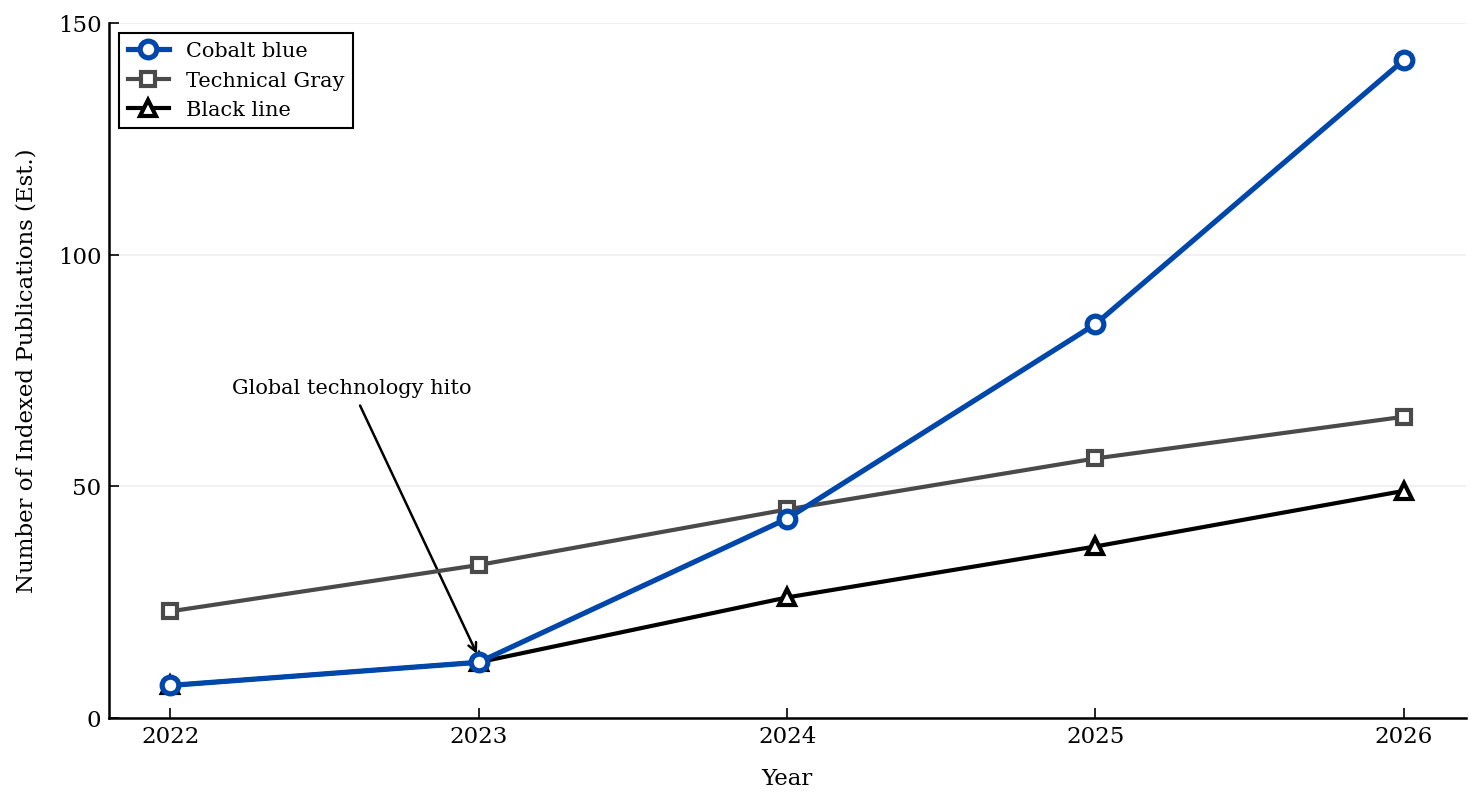
\includegraphics[width=0.95\linewidth]{fig2.png}
\scalebox{1}{\definecolor{cobaltblue}{HTML}{0047AB}
\definecolor{techgray}{HTML}{4A4A4A}

\begin{tikzpicture}
\begin{axis}[
    width=\linewidth,
    height=6.5cm,
    grid=major,
    grid style={line width=.1pt, draw=gray!20},
    xlabel={Year},
    ylabel={Number of Indexed Publications (Est.)},
    xmin=2022, xmax=2026,
    ymin=0, ymax=150,
    xtick={2022, 2023, 2024, 2025, 2026},
    ytick={0, 50, 100, 150},
    tick pos=left,
    xtick align=inside,
    ytick align=inside,
    legend pos=north west,
    % SE ELIMINÓ 'fancybox=false' PARA EVITAR EL ERROR DE COMPILACIÓN
    legend style={draw=black, fill=white, font=\footnotesize, cells={anchor=west}},
    axis x line=bottom,
    axis y line=left,
    clip=false
]

% Serie Cobalt Blue
\addplot[cobaltblue, line width=1.5pt, mark=*, mark options={fill=white, line width=1.5pt, scale=1.2}] coordinates {(2022,7)(2023,12)(2024,43)(2025,85)(2026,142)};
\addlegendentry{Cobalt blue}

% Serie Technical Gray
\addplot[techgray, line width=1.2pt, mark=square*, mark options={fill=white, line width=1.2pt, scale=1.1}] coordinates {(2022,23)(2023,33)(2024,45)(2025,56)(2026,65)};
\addlegendentry{Technical Gray}

% Serie Black Line
\addplot[black, line width=1.2pt, mark=triangle*, mark options={fill=white, line width=1.2pt, scale=1.2}] coordinates {(2022,7)(2023,12)(2024,26)(2025,37)(2026,49)};
\addlegendentry{Black line}

% Flecha y etiqueta de hito tecnológico
\draw[->, >=stealth, black, thick] (axis cs:2022.8, 65) -- (axis cs:2023, 16);
\node[black, font=\small, anchor=south east] at (axis cs:2022.9, 65) {Global technology hito};

\end{axis}
\end{tikzpicture}}
\caption{Evolución temporal de publicaciones académicas y técnicas en NTN, D2D satelital e integración TN-NTN (2021-2026).}
\label{fig:publications_evolution}
\end{figure}

En conjunto, el estado del arte muestra un progreso prometedor pero todavía fragmentado. Mientras los estándares 3GPP avanzan de forma estructurada, la verdadera convergencia TN-NTN con D2D nativo requiere soluciones que vayan más allá de la mera suma de componentes. Esta observación motiva directamente el marco arquitectónico que se desarrolla en las siguientes secciones.